
%-------------------------------------------------------------------------------}
\section{Background and Motivation}
\label{sec:background}
%-------------------------------------------------------------------------------


\subsection{All-to-All Collective in MoE}
\begin{figure}[t]
    \centering
    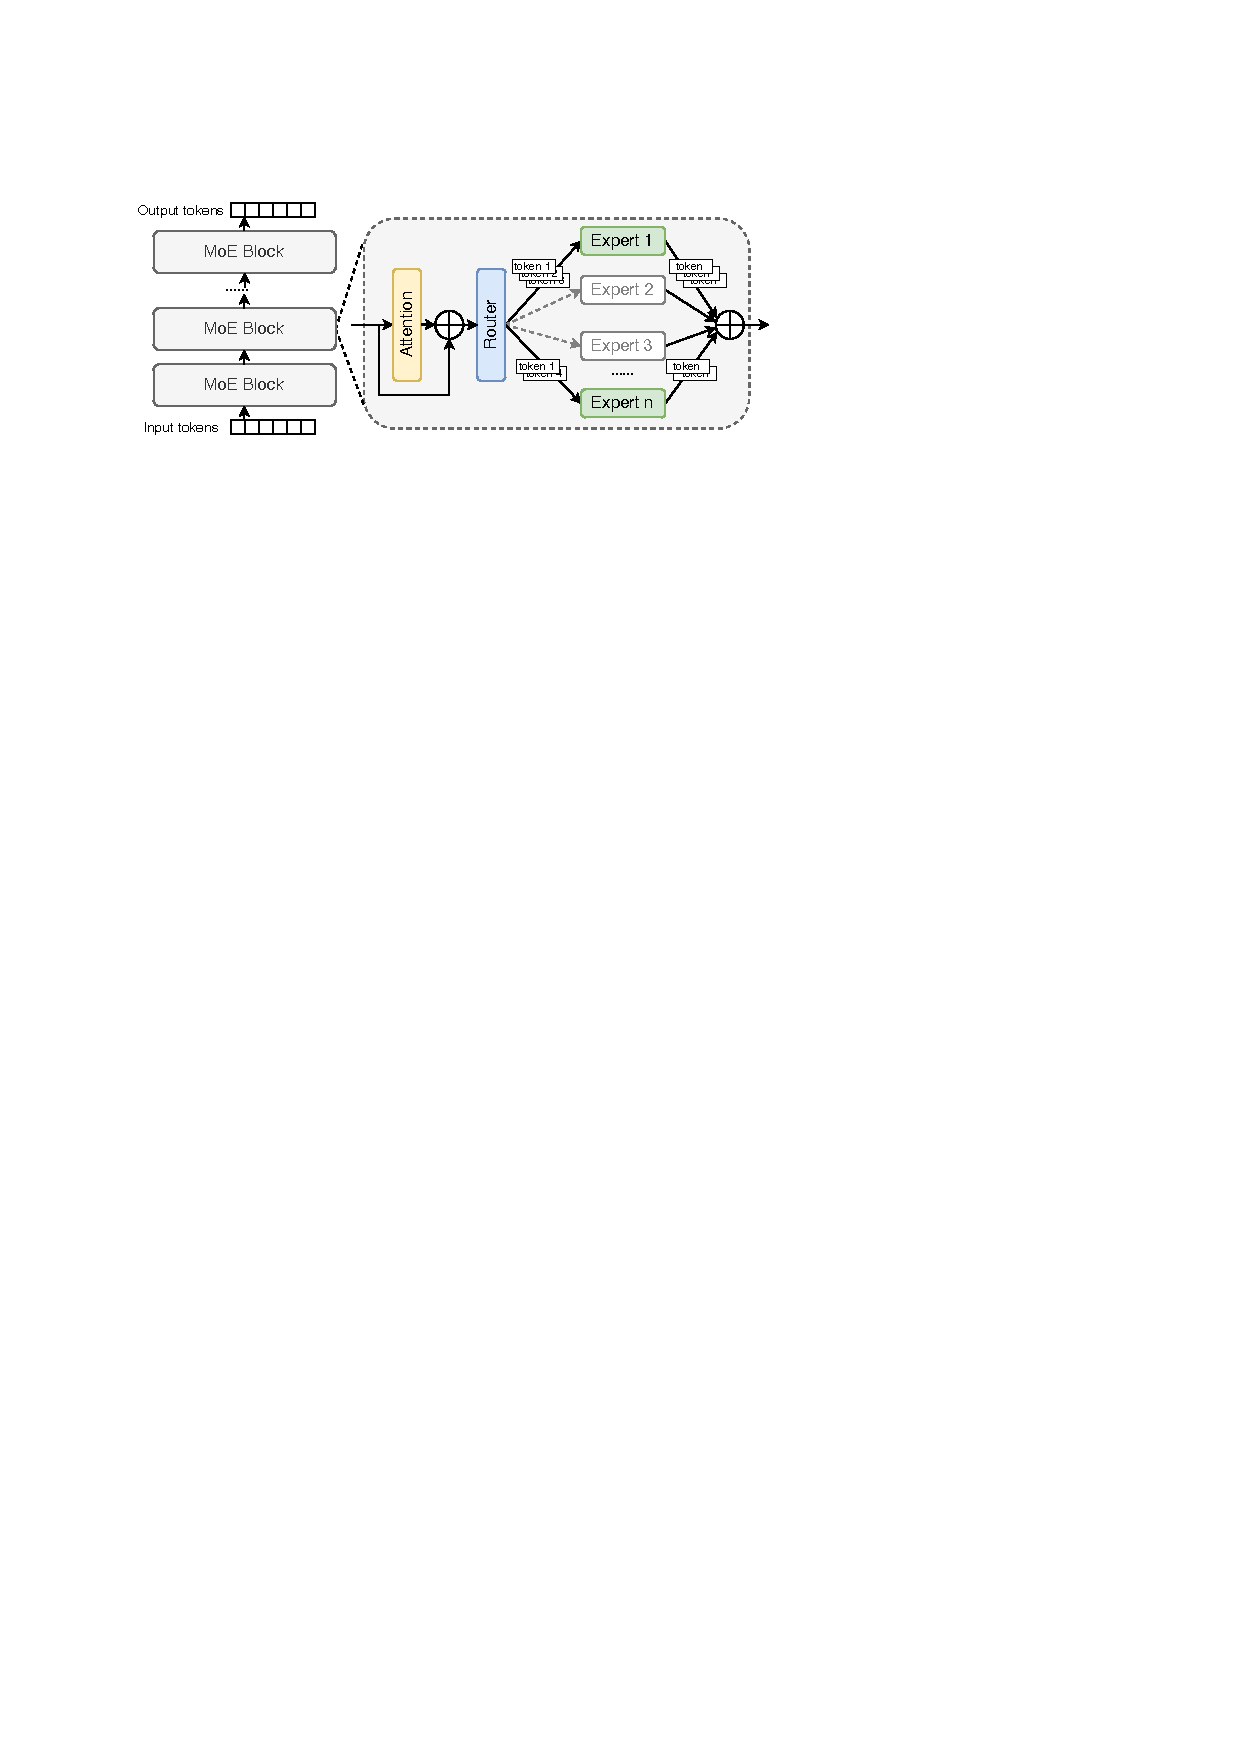
\includegraphics[width=\columnwidth]{figs/background/EP.pdf}
    \caption{Mixture-of-Experts model architecture.}
    \label{fig:EP}
    % \vspace{-0.1em}
\end{figure}

%llm dense to sparse. moe needs ep. ep workflow

Large language models (LLMs) have achieved superior performance, however, the cost of these models grows steeply with model size~\cite{megatron,llama}. To decouple model capacity from per-token computation, recent architectures increasingly adopt sparsely-activated Mixture-of-Experts (MoE) layers in place of dense feed-forward sublayers in Transformer blocks~\cite{deepseek-v3,qwen,gshard,switchtransformer}. In an MoE layer, the standard dense feed-forward sublayer is replaced by a set of $N$  expert networks, typically independent MLPs, together with a lightweight routing network. The router processes each token produced by the attention sublayer and activates only a small subset of experts to execute, as shown in Figure~\ref{fig:EP}. In practical, a single MoE layer often contains hundreds of experts, which cannot be hosted on a single GPU and are therefore distributed across multiple devices using expert parallelism~\cite{deepspeed-inference,glam,janus,undermoecomm,mixnet}. Under expert parallelism, the model partitions the expert set across a group of GPUs. A given token may thus be routed to experts residing on different GPUs within the expert-parallel group.

A forward pass through an MoE layer after attention normalization follows a three-stage pattern: token dispatch, expert computation, and result combination. First, each GPU computes for its every local token a top-\(k\) set of expert. Then bucket the tokens by expert and dispatch them to the GPUs that host the selected experts. Second, each GPU runs its resident experts, applying the expert MLP to the assigned tokens to produce updated hidden states (expert outputs) for those tokens. Finally, expert outputs are sent back to the token-owning GPUs and combined according to the routing weights to form the MoE layer's output for each token. Viewed from the communication perspective, tokens transmission between each stage naturally induces two all-to-all exchanges. Viewed from the communication perspective, the dispatch and combination stages naturally induce two all-to-all exchanges per MoE layer—one for sending routed activations and one for gathering outputs back. As this communication pattern is exercised at every MoE layer, the latency of the all-to-all collective becomes a first-order determinant of end-to-end MoE performance. Prior work reports that all-to-all communication can account for around 30\%-60\% of the total training or inference iteration time~\cite{mixnet,fusco,megascale}.






\subsection{Collective Tax}


Under an idealized model with lossless links, full pipelining, and no additional overheads, the latency of an all-to-all operation can be approximated as the ratio between the total communicated volume and the aggregate link bandwidth. Figure~\ref{fig:ccl_cost} compares the latency of MoE all-to-all collectives against this ideal baseline under different system settings and across several representative communication libraries, including NCCL~\cite{NCCL}, DeepEP~\cite{deepep}, and NVSHMEM~\cite{nvshmem}. We conduct experiments on a 4-node cluster. Each server is equipped with eight NVIDIA H800 GPUs. The detailed configuration is the same in Section~\ref{sec:evaluation}. We evaluate the single all-to-all collective latency in different expert parallelism degrees. In all cases, the observed latency exceeds the theoretical baseline, with xx\%-xx\% latency increase. This gap persists despite ample network capacity, indicating that factors beyond raw data transfer play a major role in end-to-end collective latency.

To understand where this additional latency comes from, we inspect the communication subdivisions of the collective communication libraries which is summarized in Figure~\ref{fig:codetax}. Across all evaluated libraries, all-to-all collective begins after the routing decisions are finalized. Once the gate computation completes, the expert assignment for each token becomes fixed, and an explicit synchronization point is required to ensure that all GPUs observe a consistent routing result before communication proceeds. This synchronization is common to all implementations and is necessary to preserve correctness, but it already introduces latency that is not captured by the bandwidth-bound model.

Beyond this initial synchronization, existing libraries differ significantly in how they implement the communication. In NCCL and DeepEP, all-to-all collective involves an explicit data shuffling phase both on the sender and receiver side. After gate computation, GPU SMs launch kernels that copy token data from the original tensor buffers into intermediate I/O buffers. During this copy, tokens are reorganized so that data destined for each receiver GPU occupies a contiguous memory region. This cost is independent of network transfer and is therefore invisible to a bandwidth-only performance model. A symmetric process occurs on the receiver side. Once data arrives at the destination I/O buffers, the receiving GPU launches kernels to copy data into the destination tensor buffers. This second copy is again accompanied by a layout transformation, this time to match the memory layout expected by the downstream computation kernels. As a result, a single all-to-all collective under NCCL or DeepEP typically involves memory copies and data shuffles on both the sender and receiver, even though the logical communication volume remains unchanged. After our profiling, we find that the data shuffling overhead accounts for around xx\%-xx\% of the total collective latency.

Alternatively, NVSHMEM follows a different execution path. After gate computation and synchronization, NVSHMEM enables direct remote memory access from the sender's tensor buffers to the receiver's tensor buffers, avoiding explicit data shuffling. This design eliminates intermediate I/O buffers and associated data shuffling, but relies on synchronization to coordinate access to shared tensor regions. As such, while NVSHMEM reduces shuffle-related overheads, it does not remove synchronization costs inherent to all-to-all collective. After our profiling, we find that the synchronization overhead accounts for around xx\%-xx\% of the total collective latency.

Taken together, these observations suggest that the performance gap between measured all-to-all latency and the theoretical baseline arises primarily from two sources: data shuffling due to memory layout transformations and explicit synchronization required for correct execution. Regardless of the specific implementation, however, at least one of these overheads is incurred in current all-to-all collectives. We collectively refer to the overhead beyond the theoretical baseline as the "collective tax". This tax is not specific to a particular communication library, but instead reflects a fundamental overhead of orchestrating all-to-all collective for MoE layers. Different collective paradigms pay this tax in different ways, trading off memory shuffling overhead, synchronization cost, and implementation complexity. In the next subsection, we examine how existing collective designs handle this orchestration and analyze their inherent limitations through high-level analysis.




\begin{figure}[t]
    \centering
    \includegraphics[width=0.8\columnwidth]{figs/background/ccl_cost.png}
    \caption{All-to-all collective overhead of existing collective communication libraries.}
    \label{fig:ccl_cost}
    % \vspace{-0.1em}
\end{figure}

\begin{figure}[t]
    \centering
    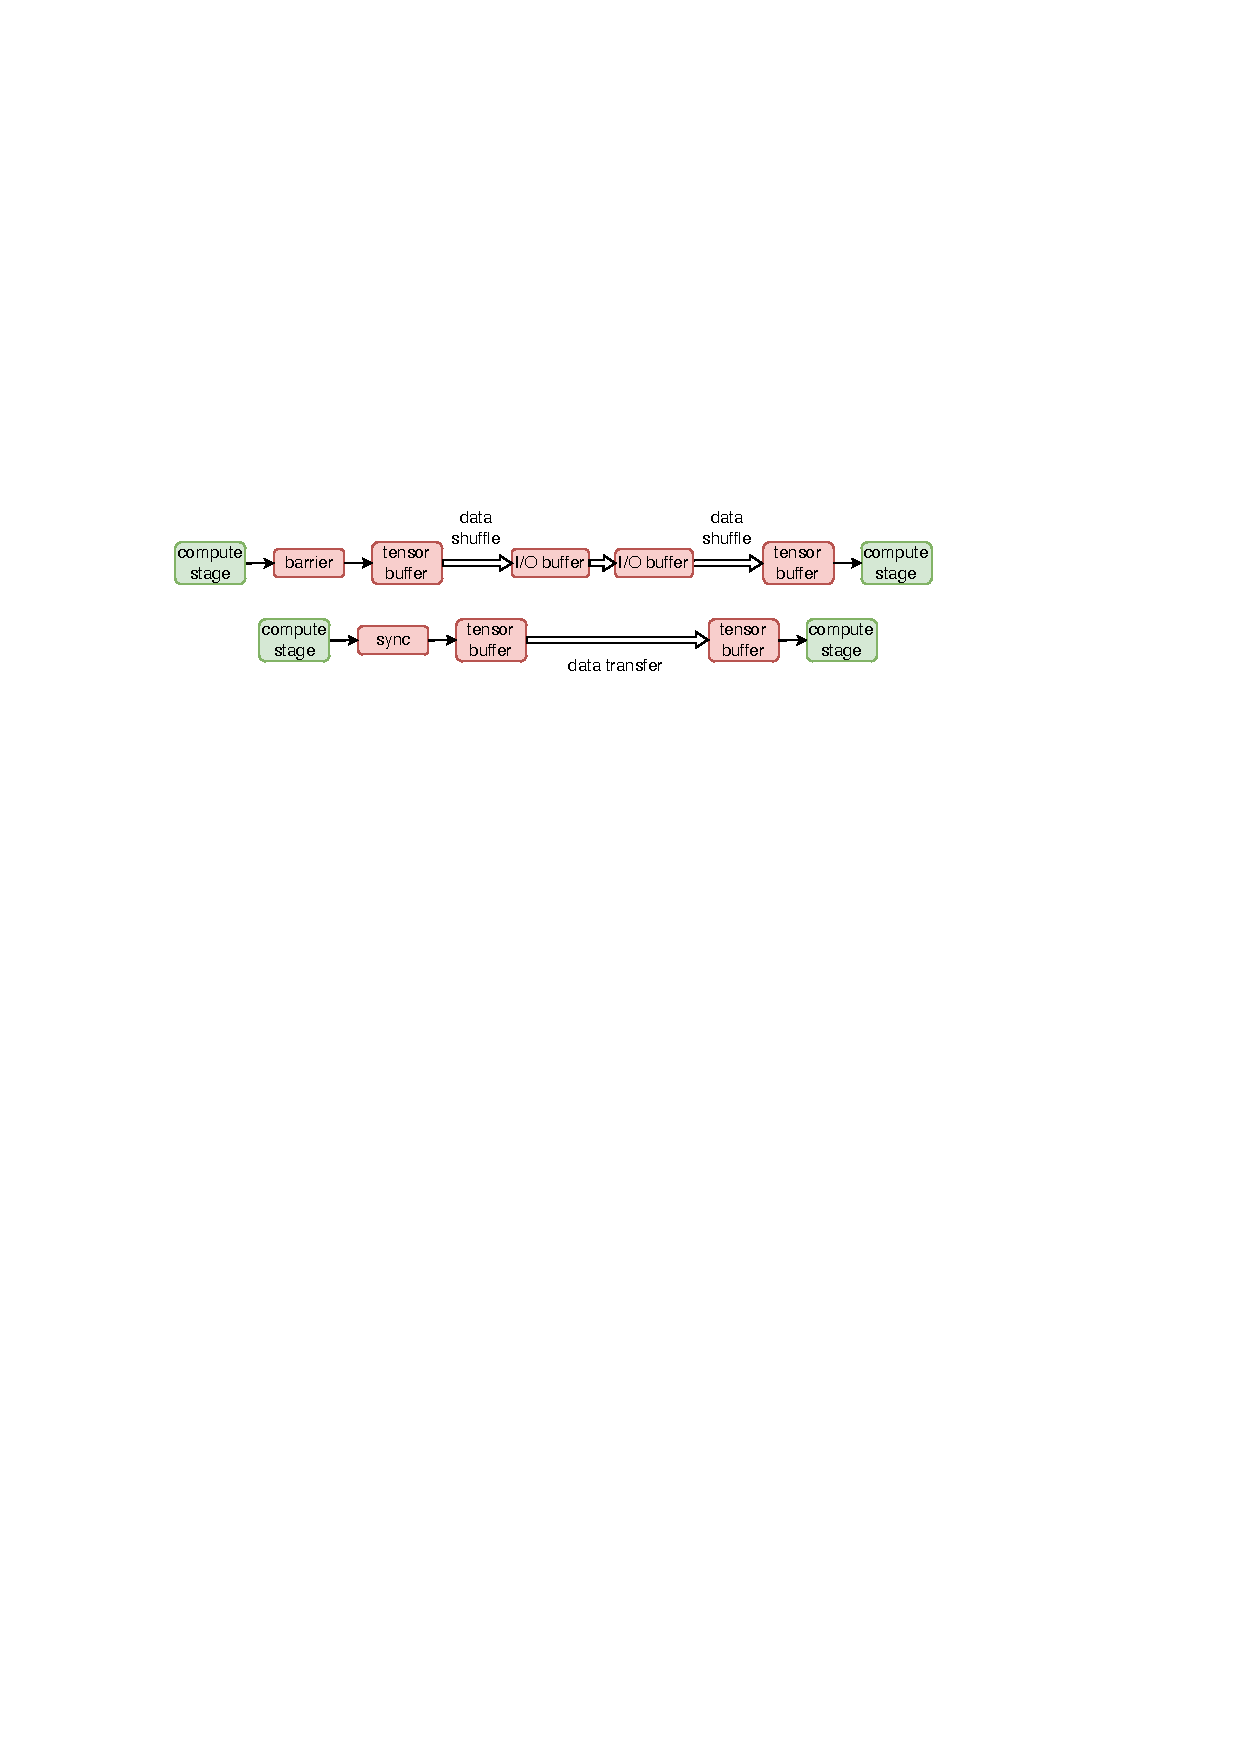
\includegraphics[width=\columnwidth]{figs/background/codetax.pdf}
    \caption{Profiled communication subdivision of different CCLs.}
    \label{fig:codetax}
    % \vspace{-0.1em}
\end{figure}




% One major source of overhead arises from memory shuffling and data rearrangement. To ensure correct placement of received data, many collective implementations require receivers to pre-allocate intermediate buffers and perform explicit data rearrangement or copying after data arrival. These memory operations consume GPU memory bandwidth and compute resources, and often serialize with kernel execution, contributing to end-to-end latency even when network transfer is complete.

% Another significant contributor is synchronization and coordination. To preserve correctness under concurrent multi-producer multi-consumer access, collective libraries frequently rely on global synchronization points, metadata exchanges, or stream-level barriers. These mechanisms are used to coordinate buffer readiness, address resolution, and write ordering across GPUs. As a result, data that has already been transferred may still be stalled waiting for synchronization, further widening the gap between measured latency and the bandwidth-bound ideal.

% We collectively refer to the overhead beyond the bandwidth-bound lower limit as collective tax. This tax is not specific to a particular communication library, but instead reflects a fundamental cost of orchestrating correct all-to-all communication for MoE inference. Different collective paradigms pay this tax in different ways, trading off memory overhead, synchronization latency, and implementation complexity. In the next subsection, we examine how existing collective designs handle this orchestration and analyze their inherent limitations through concrete case studies.



\clearpage

% \subsection{Existing Paradigms and Limitations}